\chapter{DISEÑO E IMPLEMENTACIÓN DEL INSTRUMENTO DE MEDICIÓN}

\section{Objetivo del diseño}

El presente capítulo tiene como objetivo proponer un diagrama de bloques, los criterios de selección de los componentes para cada bloque, los diagramas de flujo del programa y la implementación de la tarjeta electrónica que tendrá el instrumento de medición. Así mismo, recordar que el objetivo de la tesis es diseñar y desarrollar un instrumento de bajo costo que permita estimar la capacidad eléctrica que proveen los bancos de baterías basados en baterías Li-ion y pilas alcalinas. 

\section{Diagrama de bloques}

De acuerdo a las estructuras de los instrumentos de medición revisados en la sección 2.3 se propone el diagrama de bloques mostrado en la figura~\ref{fig:diagramabloques}.

\begin{figure}[htbp]
\centering
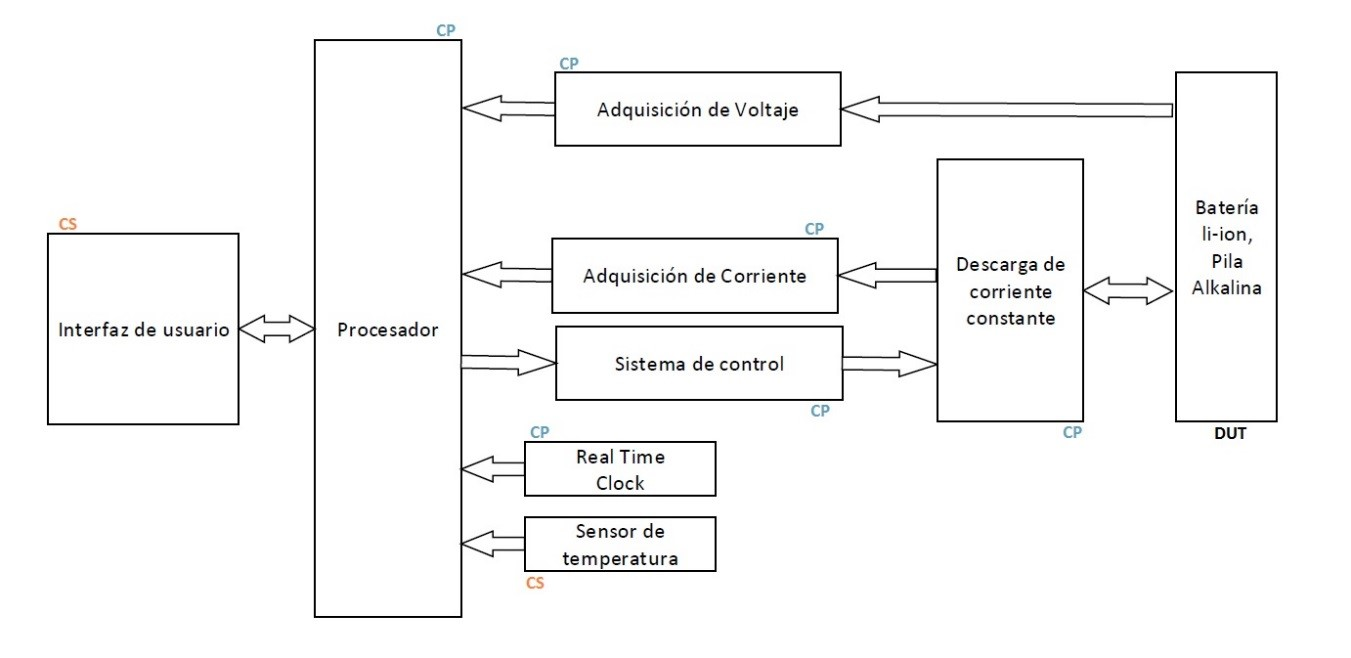
\includegraphics[width=15cm]{CAP3_diagramabloques.jpg}
\caption{Diagrama de bloques propuesto para el diseño de un instrumento de medición que estime la capacidad eléctrica de la batería}
\label{fig:diagramabloques}
\end{figure}

CP: Componente Principal	     \\
CS: Componente Secundario  \\
DUT: Dispositivio bajo prueba \\

La adquisición de datos durante la descarga de la batería es parte fundamental del sistema, por lo que se clasificará el diagrama de bloques en componentes principales y componentes secundarios. Por un lado, los componentes principales serán aquellos que influyan en cierta medida con la estimación de la capacidad eléctrica, los cuales son constituidos por los bloques: Adquisición de Voltaje, Adquisición de Corriente, Sistema de Control, Descarga de Corriente Constante, Real Time Clock y Procesador. Por otro lado, los componentes secundarios serán aquellos que no influyan en la estimación de la medida, pero si contribuirán para el adecuado desempeño del instrumento y están conformados por los bloques: Interfaz de usuario y Sensor de Temperatura. 

\textbf{\underline{Descripción del diagrama de bloques}}

La función general del diagrama de bloques comienza por el bloque de interfaz de usuario debido a que éste es el encargado de la interacción entre el instrumento y el usuario. Este bloque está conformado por periféricos de entrada y de salida, tales como: teclado numérico, display BCD 7 segmentos, display LCD 16x2, keypad 4x4, entre otros. El usuario a través estos periféricos tendrá acceso a un menú donde ingresará la corriente que desee descargar la batería. Una vez ingresado la corriente, el bloque Procesador será el encargado de tomar esta información y condicionarla para realizar la descarga de corriente constante a la batería. El bloque de Descarga de corriente constante y el bloque de Sistema de control cumplen con la función de mantener la descarga constante a pesar de las variaciones que se pueda presentar en la batería. Así mismo, mientras se va realizando la descarga, el procesador recolecta la información pertinente de la descarga por medio de los bloques de Adquisición de Voltaje y Adquisición de Corriente. El bloque de Sensor de Temperatura cada periodo de tiempo envía la información al bloque Procesador con la finalidad de saber la temperatura promedio del sistema durante toda la medición. Luego, el bloque de Real Time Clock, o también conocido como reloj externo, tiene el objetivo de brindarle al procesador los intervalos de tiempo de las adquisiciones de datos que vaya a realizar. Una vez almacenado toda esta información en memoria, el usuario a través del menú podrá acceder a la opción de transferir los datos a una computadora. 

\section{Requerimientos para el diseño}

Los requerimientos del sistema están basados según la funcionalidad que tendrá el instrumento por parte de los usuarios. En este caso, se planteó que los usuarios estén conformados por los estudiantes de la especialidad de Ingeniería Electrónica; ya que, en gran medida, los proyectos que realizan tienen una batería como fuente de alimentación. Por lo tanto, se establecen los siguientes requerimientos de las características principales del instrumento tomando como referencia la información expuesta en la sección 2.2:

\underline{Rango de voltajes de la batería:} El rango de voltajes de la batería está definido por las baterías con mayor voltaje de referencia usado en los proyectos de los estudiantes. Por lo general, las baterías de 9V son más utilizadas y con el mayor voltaje de referencia. Por ello, el rango de voltajes de la batería será de 0 a 9V.

\underline{Fuente de alimentación:} El rango de descarga de corriente debe estar entre 0 y 2A, ya que éste es el rango que manejan los bancos de baterías actualmente en el mercado.

\underline{Resolución:} Se busca que la resolución del instrumento sea la más pequeña posible, por ejemplo: 100 nA, 0.01 mA o 1 mA. Sin embargo, estas resoluciones son manejadas por instrumentos costosos en el mercado actual. Por ello, se buscará obtener al comienzo una resolución de 1 mA para que los usuarios tengan mayor precisión en el uso del instrumento.

\underline{Exactitud:} La exactitud de los instrumentos de medición representa el porcentaje de desviación de la medida realizada. Para el diseño del instrumento de la tesis, se buscará que no sea mayor al 10\% debido a que el rango de error en la adquisición de datos no debería ser considerable. 

\underline{Rango de operación de Temperatura:} El rango de operación de temperatura del instrumento será la temperatura ambiente de los laboratorios.

\underline{Interfaz de Usuario:} La interacción entre el usuario y el instrumento será entre periféricos de entrada y visualizadores. Estos periféricos de entrada pueden ser: teclado número, teclado alfanumérico, botones, entre otros. Los visualizadores deben cumplir la función de mostrar las opciones de funcionamiento del instrumento, los cuales pueden ser: display LCD 2x40, pantalla VFD 16x2, monitor externo, entre otros.

\subsection{Sistema de Control y Descarga de Corriente Constante}
\subsection{Control Digital y Adquisición de Voltaje y Corriente}
\subsection{Sensor de Temperatura e Interfaz de Usuario}
\subsection{Procesador y Reloj de Tiempo Real}
\subsection{Diagrama de Flujo}
\subsection{Implementación}
